% Created by tikzDevice version 0.12
% !TEX encoding = UTF-8 Unicode
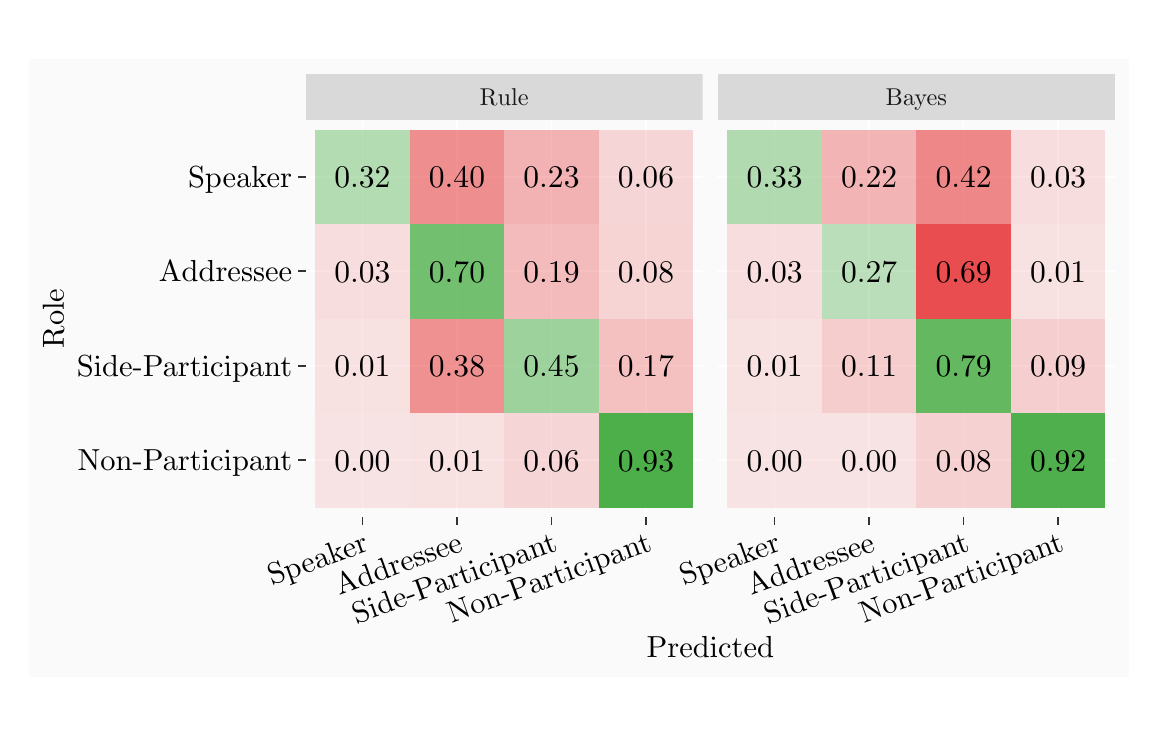
\begin{tikzpicture}[x=1pt,y=1pt]
\definecolor{fillColor}{RGB}{255,255,255}
\path[use as bounding box,fill=fillColor,fill opacity=0.00] (0,0) rectangle (398.34,246.17);
\begin{scope}
\path[clip] (  0.00, 11.09) rectangle (398.34,235.08);
\definecolor{drawColor}{RGB}{255,255,255}
\definecolor{fillColor}{gray}{0.98}

\path[draw=drawColor,line width= 0.6pt,line join=round,line cap=round,fill=fillColor] (  0.00, 11.09) rectangle (398.34,235.08);
\end{scope}
\begin{scope}
\path[clip] (100.50, 69.36) rectangle (243.92,212.78);
\definecolor{drawColor}{RGB}{255,255,255}

\path[draw=drawColor,line width= 0.6pt,line join=round] (100.50, 89.85) --
	(243.92, 89.85);

\path[draw=drawColor,line width= 0.6pt,line join=round] (100.50,123.99) --
	(243.92,123.99);

\path[draw=drawColor,line width= 0.6pt,line join=round] (100.50,158.14) --
	(243.92,158.14);

\path[draw=drawColor,line width= 0.6pt,line join=round] (100.50,192.29) --
	(243.92,192.29);

\path[draw=drawColor,line width= 0.6pt,line join=round] (120.98, 69.36) --
	(120.98,212.78);

\path[draw=drawColor,line width= 0.6pt,line join=round] (155.13, 69.36) --
	(155.13,212.78);

\path[draw=drawColor,line width= 0.6pt,line join=round] (189.28, 69.36) --
	(189.28,212.78);

\path[draw=drawColor,line width= 0.6pt,line join=round] (223.43, 69.36) --
	(223.43,212.78);
\definecolor{fillColor}{RGB}{77,175,74}

\path[fill=fillColor,fill opacity=0.40] (103.91,175.22) rectangle (138.06,209.36);
\definecolor{fillColor}{RGB}{228,26,28}

\path[fill=fillColor,fill opacity=0.48] (138.06,175.22) rectangle (172.21,209.36);
\definecolor{fillColor}{RGB}{228,26,28}

\path[fill=fillColor,fill opacity=0.32] (172.21,175.22) rectangle (206.35,209.36);
\definecolor{fillColor}{RGB}{228,26,28}

\path[fill=fillColor,fill opacity=0.16] (206.35,175.22) rectangle (240.50,209.36);
\definecolor{fillColor}{RGB}{228,26,28}

\path[fill=fillColor,fill opacity=0.13] (103.91,141.07) rectangle (138.06,175.22);
\definecolor{fillColor}{RGB}{77,175,74}

\path[fill=fillColor,fill opacity=0.78] (138.06,141.07) rectangle (172.21,175.22);
\definecolor{fillColor}{RGB}{228,26,28}

\path[fill=fillColor,fill opacity=0.28] (172.21,141.07) rectangle (206.35,175.22);
\definecolor{fillColor}{RGB}{228,26,28}

\path[fill=fillColor,fill opacity=0.17] (206.35,141.07) rectangle (240.50,175.22);
\definecolor{fillColor}{RGB}{228,26,28}

\path[fill=fillColor,fill opacity=0.11] (103.91,106.92) rectangle (138.06,141.07);
\definecolor{fillColor}{RGB}{228,26,28}

\path[fill=fillColor,fill opacity=0.47] (138.06,106.92) rectangle (172.21,141.07);
\definecolor{fillColor}{RGB}{77,175,74}

\path[fill=fillColor,fill opacity=0.53] (172.21,106.92) rectangle (206.35,141.07);
\definecolor{fillColor}{RGB}{228,26,28}

\path[fill=fillColor,fill opacity=0.26] (206.35,106.92) rectangle (240.50,141.07);
\definecolor{fillColor}{RGB}{228,26,28}

\path[fill=fillColor,fill opacity=0.10] (103.91, 72.77) rectangle (138.06,106.92);
\definecolor{fillColor}{RGB}{228,26,28}

\path[fill=fillColor,fill opacity=0.11] (138.06, 72.77) rectangle (172.21,106.92);
\definecolor{fillColor}{RGB}{228,26,28}

\path[fill=fillColor,fill opacity=0.16] (172.21, 72.77) rectangle (206.35,106.92);
\definecolor{fillColor}{RGB}{77,175,74}

\path[fill=fillColor] (206.35, 72.77) rectangle (240.50,106.92);
\definecolor{drawColor}{RGB}{0,0,0}

\node[text=drawColor,anchor=base,inner sep=0pt, outer sep=0pt, scale=  1.14] at (120.98,188.37) {0.32};

\node[text=drawColor,anchor=base,inner sep=0pt, outer sep=0pt, scale=  1.14] at (155.13,188.37) {0.40};

\node[text=drawColor,anchor=base,inner sep=0pt, outer sep=0pt, scale=  1.14] at (189.28,188.37) {0.23};

\node[text=drawColor,anchor=base,inner sep=0pt, outer sep=0pt, scale=  1.14] at (223.43,188.37) {0.06};

\node[text=drawColor,anchor=base,inner sep=0pt, outer sep=0pt, scale=  1.14] at (120.98,154.22) {0.03};

\node[text=drawColor,anchor=base,inner sep=0pt, outer sep=0pt, scale=  1.14] at (155.13,154.22) {0.70};

\node[text=drawColor,anchor=base,inner sep=0pt, outer sep=0pt, scale=  1.14] at (189.28,154.22) {0.19};

\node[text=drawColor,anchor=base,inner sep=0pt, outer sep=0pt, scale=  1.14] at (223.43,154.22) {0.08};

\node[text=drawColor,anchor=base,inner sep=0pt, outer sep=0pt, scale=  1.14] at (120.98,120.07) {0.01};

\node[text=drawColor,anchor=base,inner sep=0pt, outer sep=0pt, scale=  1.14] at (155.13,120.07) {0.38};

\node[text=drawColor,anchor=base,inner sep=0pt, outer sep=0pt, scale=  1.14] at (189.28,120.07) {0.45};

\node[text=drawColor,anchor=base,inner sep=0pt, outer sep=0pt, scale=  1.14] at (223.43,120.07) {0.17};

\node[text=drawColor,anchor=base,inner sep=0pt, outer sep=0pt, scale=  1.14] at (120.98, 85.93) {0.00};

\node[text=drawColor,anchor=base,inner sep=0pt, outer sep=0pt, scale=  1.14] at (155.13, 85.93) {0.01};

\node[text=drawColor,anchor=base,inner sep=0pt, outer sep=0pt, scale=  1.14] at (189.28, 85.93) {0.06};

\node[text=drawColor,anchor=base,inner sep=0pt, outer sep=0pt, scale=  1.14] at (223.43, 85.93) {0.93};
\end{scope}
\begin{scope}
\path[clip] (249.42, 69.36) rectangle (392.84,212.78);
\definecolor{drawColor}{RGB}{255,255,255}

\path[draw=drawColor,line width= 0.6pt,line join=round] (249.42, 89.85) --
	(392.84, 89.85);

\path[draw=drawColor,line width= 0.6pt,line join=round] (249.42,123.99) --
	(392.84,123.99);

\path[draw=drawColor,line width= 0.6pt,line join=round] (249.42,158.14) --
	(392.84,158.14);

\path[draw=drawColor,line width= 0.6pt,line join=round] (249.42,192.29) --
	(392.84,192.29);

\path[draw=drawColor,line width= 0.6pt,line join=round] (269.91, 69.36) --
	(269.91,212.78);

\path[draw=drawColor,line width= 0.6pt,line join=round] (304.05, 69.36) --
	(304.05,212.78);

\path[draw=drawColor,line width= 0.6pt,line join=round] (338.20, 69.36) --
	(338.20,212.78);

\path[draw=drawColor,line width= 0.6pt,line join=round] (372.35, 69.36) --
	(372.35,212.78);
\definecolor{fillColor}{RGB}{77,175,74}

\path[fill=fillColor,fill opacity=0.42] (252.83,175.22) rectangle (286.98,209.36);
\definecolor{fillColor}{RGB}{228,26,28}

\path[fill=fillColor,fill opacity=0.31] (286.98,175.22) rectangle (321.13,209.36);
\definecolor{fillColor}{RGB}{228,26,28}

\path[fill=fillColor,fill opacity=0.51] (321.13,175.22) rectangle (355.28,209.36);
\definecolor{fillColor}{RGB}{228,26,28}

\path[fill=fillColor,fill opacity=0.13] (355.28,175.22) rectangle (389.42,209.36);
\definecolor{fillColor}{RGB}{228,26,28}

\path[fill=fillColor,fill opacity=0.13] (252.83,141.07) rectangle (286.98,175.22);
\definecolor{fillColor}{RGB}{77,175,74}

\path[fill=fillColor,fill opacity=0.36] (286.98,141.07) rectangle (321.13,175.22);
\definecolor{fillColor}{RGB}{228,26,28}

\path[fill=fillColor,fill opacity=0.77] (321.13,141.07) rectangle (355.28,175.22);
\definecolor{fillColor}{RGB}{228,26,28}

\path[fill=fillColor,fill opacity=0.11] (355.28,141.07) rectangle (389.42,175.22);

\path[fill=fillColor,fill opacity=0.11] (252.83,106.92) rectangle (286.98,141.07);
\definecolor{fillColor}{RGB}{228,26,28}

\path[fill=fillColor,fill opacity=0.20] (286.98,106.92) rectangle (321.13,141.07);
\definecolor{fillColor}{RGB}{77,175,74}

\path[fill=fillColor,fill opacity=0.87] (321.13,106.92) rectangle (355.28,141.07);
\definecolor{fillColor}{RGB}{228,26,28}

\path[fill=fillColor,fill opacity=0.19] (355.28,106.92) rectangle (389.42,141.07);
\definecolor{fillColor}{RGB}{228,26,28}

\path[fill=fillColor,fill opacity=0.10] (252.83, 72.77) rectangle (286.98,106.92);

\path[fill=fillColor,fill opacity=0.10] (286.98, 72.77) rectangle (321.13,106.92);
\definecolor{fillColor}{RGB}{228,26,28}

\path[fill=fillColor,fill opacity=0.18] (321.13, 72.77) rectangle (355.28,106.92);
\definecolor{fillColor}{RGB}{77,175,74}

\path[fill=fillColor,fill opacity=0.99] (355.28, 72.77) rectangle (389.42,106.92);
\definecolor{drawColor}{RGB}{0,0,0}

\node[text=drawColor,anchor=base,inner sep=0pt, outer sep=0pt, scale=  1.14] at (269.91,188.37) {0.33};

\node[text=drawColor,anchor=base,inner sep=0pt, outer sep=0pt, scale=  1.14] at (304.05,188.37) {0.22};

\node[text=drawColor,anchor=base,inner sep=0pt, outer sep=0pt, scale=  1.14] at (338.20,188.37) {0.42};

\node[text=drawColor,anchor=base,inner sep=0pt, outer sep=0pt, scale=  1.14] at (372.35,188.37) {0.03};

\node[text=drawColor,anchor=base,inner sep=0pt, outer sep=0pt, scale=  1.14] at (269.91,154.22) {0.03};

\node[text=drawColor,anchor=base,inner sep=0pt, outer sep=0pt, scale=  1.14] at (304.05,154.22) {0.27};

\node[text=drawColor,anchor=base,inner sep=0pt, outer sep=0pt, scale=  1.14] at (338.20,154.22) {0.69};

\node[text=drawColor,anchor=base,inner sep=0pt, outer sep=0pt, scale=  1.14] at (372.35,154.22) {0.01};

\node[text=drawColor,anchor=base,inner sep=0pt, outer sep=0pt, scale=  1.14] at (269.91,120.07) {0.01};

\node[text=drawColor,anchor=base,inner sep=0pt, outer sep=0pt, scale=  1.14] at (304.05,120.07) {0.11};

\node[text=drawColor,anchor=base,inner sep=0pt, outer sep=0pt, scale=  1.14] at (338.20,120.07) {0.79};

\node[text=drawColor,anchor=base,inner sep=0pt, outer sep=0pt, scale=  1.14] at (372.35,120.07) {0.09};

\node[text=drawColor,anchor=base,inner sep=0pt, outer sep=0pt, scale=  1.14] at (269.91, 85.93) {0.00};

\node[text=drawColor,anchor=base,inner sep=0pt, outer sep=0pt, scale=  1.14] at (304.05, 85.93) {0.00};

\node[text=drawColor,anchor=base,inner sep=0pt, outer sep=0pt, scale=  1.14] at (338.20, 85.93) {0.08};

\node[text=drawColor,anchor=base,inner sep=0pt, outer sep=0pt, scale=  1.14] at (372.35, 85.93) {0.92};
\end{scope}
\begin{scope}
\path[clip] (100.50,212.78) rectangle (243.92,229.58);
\definecolor{fillColor}{gray}{0.85}

\path[fill=fillColor] (100.50,212.78) rectangle (243.92,229.58);
\definecolor{drawColor}{gray}{0.10}

\node[text=drawColor,anchor=base,inner sep=0pt, outer sep=0pt, scale=  0.88] at (172.21,218.15) {Rule};
\end{scope}
\begin{scope}
\path[clip] (249.42,212.78) rectangle (392.84,229.58);
\definecolor{fillColor}{gray}{0.85}

\path[fill=fillColor] (249.42,212.78) rectangle (392.84,229.58);
\definecolor{drawColor}{gray}{0.10}

\node[text=drawColor,anchor=base,inner sep=0pt, outer sep=0pt, scale=  0.88] at (321.13,218.15) {Bayes};
\end{scope}
\begin{scope}
\path[clip] (  0.00,  0.00) rectangle (398.34,246.17);
\definecolor{drawColor}{gray}{0.20}

\path[draw=drawColor,line width= 0.6pt,line join=round] (120.98, 66.61) --
	(120.98, 69.36);

\path[draw=drawColor,line width= 0.6pt,line join=round] (155.13, 66.61) --
	(155.13, 69.36);

\path[draw=drawColor,line width= 0.6pt,line join=round] (189.28, 66.61) --
	(189.28, 69.36);

\path[draw=drawColor,line width= 0.6pt,line join=round] (223.43, 66.61) --
	(223.43, 69.36);
\end{scope}
\begin{scope}
\path[clip] (  0.00,  0.00) rectangle (398.34,246.17);
\definecolor{drawColor}{RGB}{0,0,0}

\node[text=drawColor,rotate= 20.00,anchor=base east,inner sep=0pt, outer sep=0pt, scale=  1.10] at (123.58, 57.29) {Speaker};

\node[text=drawColor,rotate= 20.00,anchor=base east,inner sep=0pt, outer sep=0pt, scale=  1.10] at (157.72, 57.29) {Addressee};

\node[text=drawColor,rotate= 20.00,anchor=base east,inner sep=0pt, outer sep=0pt, scale=  1.10] at (191.87, 57.29) {Side-Participant};

\node[text=drawColor,rotate= 20.00,anchor=base east,inner sep=0pt, outer sep=0pt, scale=  1.10] at (226.02, 57.29) {Non-Participant};
\end{scope}
\begin{scope}
\path[clip] (  0.00,  0.00) rectangle (398.34,246.17);
\definecolor{drawColor}{gray}{0.20}

\path[draw=drawColor,line width= 0.6pt,line join=round] (269.91, 66.61) --
	(269.91, 69.36);

\path[draw=drawColor,line width= 0.6pt,line join=round] (304.05, 66.61) --
	(304.05, 69.36);

\path[draw=drawColor,line width= 0.6pt,line join=round] (338.20, 66.61) --
	(338.20, 69.36);

\path[draw=drawColor,line width= 0.6pt,line join=round] (372.35, 66.61) --
	(372.35, 69.36);
\end{scope}
\begin{scope}
\path[clip] (  0.00,  0.00) rectangle (398.34,246.17);
\definecolor{drawColor}{RGB}{0,0,0}

\node[text=drawColor,rotate= 20.00,anchor=base east,inner sep=0pt, outer sep=0pt, scale=  1.10] at (272.50, 57.29) {Speaker};

\node[text=drawColor,rotate= 20.00,anchor=base east,inner sep=0pt, outer sep=0pt, scale=  1.10] at (306.65, 57.29) {Addressee};

\node[text=drawColor,rotate= 20.00,anchor=base east,inner sep=0pt, outer sep=0pt, scale=  1.10] at (340.79, 57.29) {Side-Participant};

\node[text=drawColor,rotate= 20.00,anchor=base east,inner sep=0pt, outer sep=0pt, scale=  1.10] at (374.94, 57.29) {Non-Participant};
\end{scope}
\begin{scope}
\path[clip] (  0.00,  0.00) rectangle (398.34,246.17);
\definecolor{drawColor}{RGB}{0,0,0}

\node[text=drawColor,anchor=base east,inner sep=0pt, outer sep=0pt, scale=  1.10] at ( 95.55, 86.06) {Non-Participant};

\node[text=drawColor,anchor=base east,inner sep=0pt, outer sep=0pt, scale=  1.10] at ( 95.55,120.21) {Side-Participant};

\node[text=drawColor,anchor=base east,inner sep=0pt, outer sep=0pt, scale=  1.10] at ( 95.55,154.35) {Addressee};

\node[text=drawColor,anchor=base east,inner sep=0pt, outer sep=0pt, scale=  1.10] at ( 95.55,188.50) {Speaker};
\end{scope}
\begin{scope}
\path[clip] (  0.00,  0.00) rectangle (398.34,246.17);
\definecolor{drawColor}{gray}{0.20}

\path[draw=drawColor,line width= 0.6pt,line join=round] ( 97.75, 89.85) --
	(100.50, 89.85);

\path[draw=drawColor,line width= 0.6pt,line join=round] ( 97.75,123.99) --
	(100.50,123.99);

\path[draw=drawColor,line width= 0.6pt,line join=round] ( 97.75,158.14) --
	(100.50,158.14);

\path[draw=drawColor,line width= 0.6pt,line join=round] ( 97.75,192.29) --
	(100.50,192.29);
\end{scope}
\begin{scope}
\path[clip] (  0.00,  0.00) rectangle (398.34,246.17);
\definecolor{drawColor}{RGB}{0,0,0}

\node[text=drawColor,anchor=base,inner sep=0pt, outer sep=0pt, scale=  1.10] at (246.67, 18.53) {Predicted};
\end{scope}
\begin{scope}
\path[clip] (  0.00,  0.00) rectangle (398.34,246.17);
\definecolor{drawColor}{RGB}{0,0,0}

\node[text=drawColor,rotate= 90.00,anchor=base,inner sep=0pt, outer sep=0pt, scale=  1.10] at ( 13.08,141.07) {Role};
\end{scope}
\end{tikzpicture}
